\chapter{OPTIMIZATION PROBLEM}
\section{Knapsack Problem:}
The knapsack problem (KP) can be formally defined as follows: Given an instance of the knapsack problem with item set $N$, consisting of $n$ items, $N:=\left\{ 1,..., n \right\}$ j with profit $p_{j}$ and weight $w_{j}$, and the capacity value c, (Usually, all those values are taken from the positives integer numbers.) Then the objective is to select a subset of $N$ such that the total profit of the selected items is maximized and the weights does not exceed c.\\
Alternatively, a knapsack can be formulated as a solution of the following linear integer programming formulation:
\begin{subequations}
\renewcommand{\theequation}{\arabic{parentequation}--\arabic{equation}}
\begin{align}
    (KP)\hspace{1cm}&
    \text{maximize}\sum_{j=1}^{n}p_{j}x_{j}\\
    &\text{subject}\sum_{j=1}^{n}w_{j}x_{j}\le c,\\
    &x_{j}\in \left\{ 0, 1 \right\}, j=1,..., n.
\end{align}
\end{subequations}
The two functions (1.1) and (1.2) define the objective (maximize the profit) and the constraint (the total weight does not exceed c) respectively.\\
Such:\\
$\bullet$ $x_{j}$ is a binary value, which means $x_{j}=1$ if we put the item j into the knapsack and $x_{j}=0$ if we don't.\\
$\bullet$ j refers to the item, $j\le n$.
\section{Multi-Dimensional Knapsack Problem MDKP:}
We given a knapsack with m-dimensions, let $b_{i}$ be the capacity of the ith dimension, $i=1, 2, ..., m$. There are n items, and let $u_{j}$ be the number of copies of item $j, j=1, 2, ..., n$, the jth item requires $a_{ij}$ units of the ith dimension of the knapsack. The reward of including a single copy of item j in the knapsack is $c_{j}$. The problem can formulated as follows:
\begin{subequations}
\renewcommand{\theequation}{\arabic{parentequation}--\arabic{equation}}
\begin{align}
    maxZ=&\sum_{j=1}^{n}c_{j}x_{j}\\    \text{subject to}& \sum_{j=1}^{n}a_{ij}x_{j}\le b_{i},\hspace{1cm}i=1, 2,..., m,
\end{align}
\end{subequations}
\newpage
\section{Multi-dimensional Multi-choice Knapsack Problem (MMKP):}
We have n groups of items. Group i has $l_{i}$ items. Each item of the group has a particular value and it requires m resources. The objective of (MMKP) is pick exactly one item from each group for maximum total value of the collected items in mathematical notation,  let $v_{ij}$ and $\overrightarrow{r_{ij}}=\left( r_{ij1}, r_{ij2}, ..., r_{ijm} \right)$ be the value (profit) and required resource vector of the object $o_{ij}$, i.e., jth of the ith group. Also assume that $\overrightarrow{R}=\left( R_{1}, R_{2}, ..., R_{m} \right)$ be the resource bound of the knapsack \cite{iqbal2010solving}.
 Now, the problem is to
\begin{subequations}
\renewcommand{\theequation}{\arabic{parentequation}--\arabic{equation}}
\begin{align}
    (KP)\hspace{1cm}&
    \text{maximize}\sum_{j=1}^{n}p_{j}x_{j}\\
    &\text{subject\hspace{.6cm}}\sum_{j=1}^{n}w_{j}x_{j}\le c,\\
    &x_{j}\in \left\{ 0, 1 \right\}, j=1,..., n.
\end{align}
\end{subequations}
where 


$k=1, 2,..., m, x_{ij}$



in $\left\{0, 1\right\}$



 are the picking variables, and for all $i\in 1 \text{ to n, }\sum_{j=1}^{l_{i}}x_{ij}=1.$\\
Figure 1 illustrate a MMKP, We have to pick exactly one item from each group. Each item has two resources, $r_{1} \text{ and }r_{2}$. Clearly we must satisfy $\sum\text{(}r_{1}\text{  of picked items)}\le17 \text{ and }\sum\text{(}r_{2}\text{ of picked items)}\le15$ and maximize the total value of picked items.
\begin{figure}[H]
	\begin{center}
		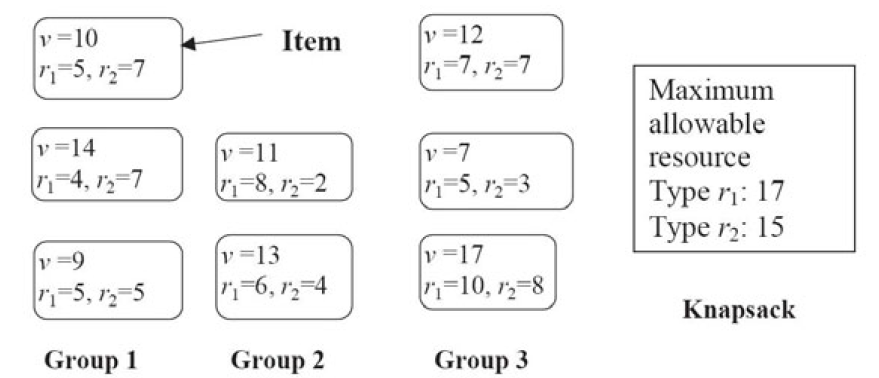
\includegraphics[scale=0.5]{fig1.png}
		\caption{Multi-dimension Multi-choice Knapsack Problem}
	\end{center}
\end{figure}
\bibliographystyle{plain}
\bibliography{sample.bib}